\documentclass[../main.tex]{subfiles}
\graphicspath{{\subfix{../Images/}}}

\begin{document}

\chapter{Chapter 9. Advanced Topics}

This chapter covers advanced Cg usage and has the following five sections:

\begin{itemize}
\item \textbf{"Fog"} describes how to simulate a common atmospheric effect that looks like fog.
\item \textbf{"Nonphotorealistic Rendering"} describes a field of rendering that focuses on stylized images, and it gives an example in the form of cartoon shading.
\item \textbf{"Projective Texturing"} explains the theory and practice of projecting textures onto geometry.
\item \textbf{"Shadow Mapping"} shows a common way to add shadows to your scenes, based on projective texturing.
\item \textbf{"Compositing"} describes how to leverage the GPU's powerful texture mapping capabilities to combine images.
\end{itemize}

\section{9.1 Fog}

Fog, an atmospheric effect created by condensed water vapor, obscures visibility. Haze, mist, and smoke are similar phenomena created by particles suspended in the air. Our treatment of these effects is similar, so we will use the blanket term \textit{fog} to refer to this broad range of atmospheric effects.

Computer graphics scenes, particularly outdoor environments, look abnormally sharp and clear without fog. Fog adds realism and character to renderings. Plus, it improves performance when it's combined with application-driven culling of fully fogged distant features, such as mountains. If an object is sufficiently distant, it is totally obscured by the fog and does not need to be rendered.

In this section, you will learn how to implement one version of fog called \textit{uniform fog}, which is illustrated in Figure \ref{fig:9-1}. The left panel of the figure shows a basic city model without fog. In the right panel, uniform fog has been added to the scene, making the distant buildings look faded. In fact, one building is far enough away that the fog completely hides it. In such a situation, you could improve performance by using a lower level of detail for the distant buildings and leaving out the totally obscured building.

\begin{figure}
    \centering
    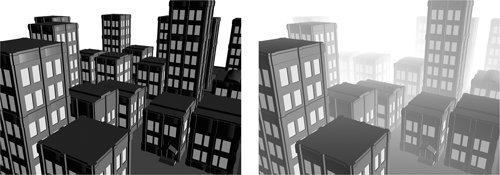
\includegraphics[width=1\linewidth]{fig9_1.jpg}
    \caption{Figure 9-1 Adding Uniform Fog to a Scene}
    \label{fig:9-1}
\end{figure}

\subsection{9.1.1 Uniform Fog}

Along a particular ray from some object to your eye, fog particles suspended in the air "scatter" some of the light that would otherwise reach your eye. Pollutants, smoke, and other airborne particles can also absorb light, rather than scattering the light, thereby reducing the intensity of the light that reaches your eye.

Whereas some light that travels along the ray is absorbed or scattered away, fog particles can redirect other scattered light, so that \textit{extra} light reaches your eye along the same ray. This redirected light comes from the aggregate scattering of light by the fog particles. Figure \ref{fig:9-2} shows the different ways that light travels from one point to another, depending on the presence of fog. If no fog particles intervene, the light rays go directly from point A to point B. If, however, there are fog particles in the air, then they may absorb or scatter some of the light, and additionally redirect random light rays from aggregate scattering toward point B.

\begin{figure}
    \centering
    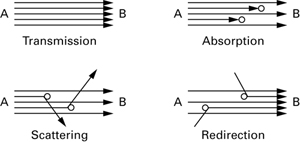
\includegraphics[width=0.75\linewidth]{fig9_2.jpg}
    \caption{Figure 9-2 Fog Particles May Affect Light Traveling from Point A to Point B}
    \label{fig:9-2}
\end{figure}

When the light is scattered by water vapor, the color of this aggregate scattered and redirected light tends to be dull white. When the scattering is due to pollution or smoke suspended in the air, the color can vary from gray for haze to black for thick smoke.

The farther the light travels along the ray from the viewed object to your eye, the greater the possibility that fog particles will scatter or extinguish light. At the same time, there is a greater opportunity to redirect extra light along the ray toward the eye. This is why fog is more apparent in the distance.

\subsection{9.1.2 The Attributes of Fog}

\begin{itemize}
\item The aggregate color of the scattered light that reaches your eye is the \textit{fog color}.
\item The measure of how much light is scattered or extinguished by fog over a given unit of distance on a view ray is the \textit{fog density}. The greater the fog density, the thicker the fog appears.
\item The distance along the view ray from an object to the eye is the \textit{fog distance}. The larger the fog distance, the foggier an object appears.
\end{itemize}

For now, assume that the fog density and fog color are uniform and constant, but let the fog distance from the eye to a visible object vary. What we want to know, and what we want to compute with Cg, is how fog affects the apparent color of distant objects under these foggy conditions.

\subsection{9.1.3 The Mathematics of Fog}

\subsection*{Absorption, Scattering, and Redirection over a Unit Distance}

If light travels a unit of distance along some ray through a uniformly foggy atmosphere, you can reason mathematically that the fog reduces the intensity of the light by some constant percentage because of absorption and scattering. At the same time, light redirected in the direction of the ray increases the intensity of the light. The following equation expresses this:

\FloatBarrier
$
C_{leave}=C_{enter}-C_{reduction}+C_{increase}
$
\FloatBarrier

where:

\begin{itemize}
\item $C_{leave}$ is the color intensity of the light leaving a unit segment along a ray,
\item $C_{enter}$ is the color intensity of the light entering a unit segment along a ray,
\item $C_{reduction}$ is the color intensity of all the light absorbed or scattered away along the unit segment, and
\item $C_{increase}$ is the color intensity of additional light redirected by the fog in the direction of the ray along the unit segment.
\end{itemize}

The intensity of light absorbed or scattered away cannot be greater than the intensity of incoming light. Assuming a uniform fog density, there must be a fixed ratio between the color of incoming light and the color of light scattered away. So we have:

\FloatBarrier
$
0\leq C_{reduction}\leq C_{enter} \newline
C_{reduction}=h\times C_{enter} \newline
0\leq h\leq 1
$
\FloatBarrier

where:
\begin{itemize}
\item $h$ is a constant scale factor dependent on the fog density.
\end{itemize}

Assuming a uniform fog color, the color of additional light scattered by the fog in the direction of the ray is:

\FloatBarrier
$
C_{increase}=h\times C_{fog}
$
\FloatBarrier

where:
\begin{itemize}
\item $C_fog$ is the constant fog color.
\end{itemize}

Now you can express the color of the light leaving the fogged unit distance in terms of the color of the entering light, a constant percentage of light scattering and extinction, and a constant fog color. This relationship is:

\FloatBarrier
$
C_{leave}=(1-h)\times C_{enter}+h\times C_{fog}
$
\FloatBarrier

\subsection*{Expressing Fog As a Linear Blend}

You can rearrange this equation as a linear blend, where $g = 1 - h$, so it then reads:

\FloatBarrier
$
C_{leave}=g\times C_{enter}+(1-g)\times C_{fog}
$
\FloatBarrier

This means that the intensity of the light at the end of the unit distance "fogged ray segment" is equal to the initial intensity of the light at the beginning of the segment, reduced by some fraction $g$ of the initial light intensity, but increased by the fraction $(1 - g)$ of the fog color.

\subsection*{Applying Fog over Multiple Units of Distance}

We can apply the formula recursively if the fog travels multiple units of distance, assuming that the fog density and color are uniform over all those units of distance. When the light travels three unit distances, the intensity of the light at the end of the three-unit ray is:

\FloatBarrier
$
C_{leave}=g\times (g\times (g\times C_{enter}+(1-g)\times C_{fog})+(1-g)\times C_{fog})+(1-g)\times C_{fog}
$
\FloatBarrier

This simplifies to the following:

\FloatBarrier
$
C_{leave}=g^3\times C_{enter}+(1-g^3)\times C_{fog}
$
\FloatBarrier

Notice how we raise $g$ to the third power in the course of applying fog over three units of distance. We generalize this function for an arbitrary fog distance $z$ as:

\FloatBarrier
$
C_{eye}=g^z\times C_{object}+(1-g^z)\times C_{fog}
$
\FloatBarrier

Our true interest is the color of an object as seen by the eye looking through the fog, rather than merely two points at the beginning and end of an arbitrary ray, so we have relabeled $C_{leave}$ as $C_{eye}$ and $C_{enter}$ as $C_{object}$.

Recall that you can rewrite an exponential such as $g^z$ in terms of exponential and logarithmic functions, so:

\FloatBarrier
$
g^z=exp_2(log_2(g)\times z)
$
\FloatBarrier

Expressing $C_{eye}$ in terms of exponential and logarithmic functions results in Equation 9-1.

\FloatBarrier
\begin{equationcaption}
$
C_{eye}=f\times C_{object}+(1-f)\times C_{fog} \newline
f=exp_2(-d\times z) \newline
d=-log_2(g)
$
\caption{Equation 9-1 Uniform Fog}
\end{equationcaption}
\FloatBarrier

We call $z$ the fog distance, $d$ the fog density, and $f$ the fog factor. What base you choose for the exponential and logarithmic functions does not matter as long as the base is the same for both.

\begin{framed}
CineFX

CineFX GPUs efficiently compute the base 2 exponential and logarithmic functions ($exp_2$ and $log_2$). For optimal performance, use the \textbf{exp2} and \textbf{log2} Cg Standard Library routines to compute these functions.
\end{framed}

The exponential nature of the equation for computing the fog factor makes sense when you consider that for every unit of distance that light travels through fog, a certain percentage of the incoming intensity is scattered. This is similar to the process of radioactive decay of an isotope that is modeled by an exponential decay function.

We assume that the fog density $d$ and fog distance $z$ (an absolute distance) are nonnegative. The negation of $d$ in the computation of the fog factor ensures exponential decay, rather than growth.

\subsection{9.1.4 Intuiting the Equations}

To make sure that the previous equations match our intuition about how fog works, consider what happens when the fog distance $z$ is 0, or very close to 0. In this case, the object is very close to the eye and we expect zero, or very little, fog. If $z = 0$, then:

\FloatBarrier
$
f=exp_2(-d\times 0)=1
$
\FloatBarrier

and therefore the eye sees all (100 percent) of the object color and none (0 percent) of the fog color, as expected.

If the fog distance $z$ is very large, then:

\FloatBarrier
$
f=exp_2(-d\times \infty)\approx exp(-\infty)=0
$
\FloatBarrier

so the eye sees none of the object color and all of the fog color. This makes sense because fog obscures distant objects.

The larger the magnitude of the fog density $d$, the thicker the fog becomes. Likewise, small values of $d$ reduce the fog. If $d$ is 0, then:

\FloatBarrier
$
f=exp_2(-0\times z)=1
$
\FloatBarrier

which means that the color of the object is 100 percent of the object color and 0 percent of the fog color.

\subsection{9.1.5 Creating Uniform Fog with Cg}

The Cg programs that follow implement the theory of fog as we've explained it in the preceding discussion.

Example 9-1's \textbf{C9E1f_fog} fragment program implements the fog equation presented in Section 9.1.3, specifically. The program samples a decal texture; modulates the decal color with the interpolated color; and fogs the textured fragment color, assuming an interpolated fog exponent and a uniform fog color.

\begin{framed}
CineFX

The \textbf{C9E1f_fog} program is a good example of a situation in which the \textbf{fixed} data type improves performance on CineFX GPUs. Math operations such as three-component and four-component multiplies and \textbf{lerp} functions are more efficient when performed on \textbf{fixed} quantities on CineFX GPUs. Also, the \textbf{C9E1f_fog} fragment program relies on the \textbf{exp2} Standard Library routine, supported only by advanced fragment profiles.
\end{framed}

The \textbf{C9E1f_fog} fragment program is meant to be combined with the vertex program shown in Example 9-2. The \textbf{C9E2v_fog} program computes a fog exponent from the shortest distance to the eye (computed with the \textbf{length} Standard Library function) and the uniform \textbf{fogDensity} parameter.

Other quality improvements and performance optimizations are possible.

\FloatBarrier
\begin{lstlisting}[caption=Example 9-1. The \textbf{C9E1f_fog} Fragment Program]
void C9E1f_fog(float2 texCoord    : TEXCOORD0,
               float  fogExponent : TEXCOORD1,
               float4 color       : COLOR,

           out float4 oColor : COLOR,

       uniform sampler2D decal,
       uniform float3 fogColor)
{
  float fogFactor   = exp2(-abs(fogExponent));
  float4 decalColor = tex2D(decal, texCoord);
  float4 texColor   = color * decalColor;

  oColor.xyz = lerp(fogColor, texColor.xyz,
                    fogFactor);
  oColor.w = color.w;
}
\end{lstlisting}
\FloatBarrier

\FloatBarrier
\begin{lstlisting}[caption=Example 9-2. The \textbf{C9E2v_fog} Vertex Program]
void C9E2v_fog(float4 position     : POSITION,
               float4 color        : COLOR,
               float2 decalCoords  : TEXCOORD0,

           out float4 oPosition    : POSITION,
           out float4 oColor       : COLOR,
           out float2 oDecalCoords : TEXCOORD0,
           out float  fogExponent  : TEXCOORD1,

       uniform float    fogDensity,  // Based on log2
       uniform float4x4 modelViewProj,
       uniform float4x4 modelView)
{
  // Assume nonprojective modelview matrix
  float3 eyePosition = mul(modelView, position).xyz;
  float fogDistance  = length(eyePosition);
  fogExponent  = fogDistance * fogDensity;
  oPosition    = mul(modelViewProj, position);
  oDecalCoords = decalCoords;
  oColor       = color;
}
\end{lstlisting}
\FloatBarrier

\subsection*{Planar Fog Distance}

Computing the planar eye distance, rather than the Euclidean eye distance, requires fewer vertex program operations. Instead of using the \textbf{length} routine to compute the \textbf{fogDistance}, use the following planar fog distance alternative, which is often acceptable:

\FloatBarrier
\begin{lstlisting}
   float fogDistance = eyePosition.z;
\end{lstlisting}
\FloatBarrier

For very wide angles of view, this approximation can lead to an inadequate amount of fog in the far edges of the field of view, but it usually works quite well.

\subsection*{Per-Fragment Euclidean Fog Distance}

Instead of interpolating a Euclidean distance, uniform fog is more accurate if the vertex program outputs 3D eye-space coordinates that the rasterizer interpolates linearly. The fragment program then computes the true Euclidean distance at every fragment prior to computing the fog exponent and the rest of the fog computation. Although this approach is more accurate, the expense of this technique usually outweighs the quality benefit for reasonably well tessellated scenes.

\subsection*{Encoding the Fog Factor Conversion Function in a Texture}

Rather than using the Cg Standard Library's \textbf{exp2} (or similar) exponential function, your custom fog implementation can encode the function that converts the fog exponent, or distance, to a fog factor as a 1D, 2D, or 3D texture. Texture accesses are often efficient and give you more control of the fog fall-off. Keep in mind that you will need to scale the fog distance to match the [0, 1] range of the texture image.

\section{9.2 Nonphotorealistic Rendering}

Most shader authors try to create continually improving representations of reality with their computer-generated images. In fact, the majority of this book has focused on this objective. We started with simple concepts and gradually added more and more complicated effects—all with the goal of teaching you how to produce more realistic shaders.

Sometimes, however, you want to produce images that \textit{don't} look real. In a computer-aided design (CAD) program, you might want to represent objects in wireframe, or with flat shading, so that their shape is easily discernible. In a physically based rocket simulation, you might color an area of the rocket to represent its temperature instead of its physical appearance. Or perhaps you want to create cartoons.

All these examples fall under an area called \textit{nonphotorealistic rendering}, or NPR. In NPR, the idea is to stylize renderings in a specific way, so that their value comes from something other than representing them as they would look in the "real world."

\subsection{9.2.1 Toon Shading}

A complete survey of the NPR world is beyond the scope of this book, but we will look at a common and useful NPR technique called \textit{toon shading}. Toon shading is a rendering technique that shades objects with constant, sharply delineated colors—as if they were cartoons instead of real-world objects.

Figure \ref{fig:9-3} gives you an idea of the results you can achieve with toon shading. The left side of the figure shows a ray gun with ordinary diffuse and specular lighting; the right side shows an equivalent toon-shaded version. The surfaces on the toon-shaded ray gun are shaded with just three tones: one for bright diffuse regions, another for dark diffuse regions, and a third for specular highlights. Also, note that the toon-shaded ray gun is outlined in black.

\begin{figure}
    \centering
    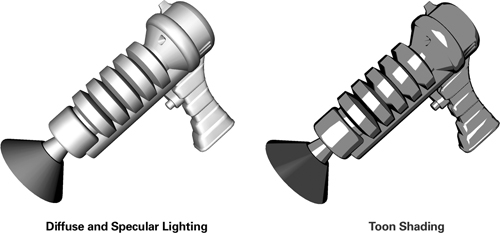
\includegraphics[width=1\linewidth]{fig9_3.jpg}
    \caption{Figure 9-3 Toon Shading}
    \label{fig:9-3}
\end{figure}

A very useful aspect of toon shading is that you don't have to change how you represent your characters and objects. Instead of drawing everything as two-dimensional images (or \textit{sprites}), you continue to draw them as three-dimensional meshes. The trick is in shading them. By replacing a conventional lighting shader with a new kind of shader, you can make these renderings look like cartoons.

\subsection{9.2.2 Implementing Toon Shading}

Most of the time, lighting is used to give an object a realistic, shaded appearance. For toon shading, however, the goal is to reduce the variation in shading.

Your toon shader has three main components:

\begin{enumerate}
\item The diffuse shading needs to be represented by just two values: one for bright regions, and another for dark regions.
\item Specular highlights need to be identified and represented as a single color where their intensity is sufficiently high.
\item Objects need to be outlined to complete the cartoon look.
\end{enumerate}

\subsection{Diffuse Shading}

A toon shader needs to convert diffuse lighting from many shades of color into just a few. Think of a monochromatic example with diffuse lighting, where every pixel has a color that ranges from 0.0 to 1.0. Because of the diffuse lighting, the values in the pixels usually vary gradually from 0.0 (in unlit regions) to 1.0 (in fully lit regions).

One way to create a toon shader would be to divide this continuous range into two distinct ranges. For example, you could take pixels with values from 0.0 to 0.5 and represent those with 0.2, and take pixels with values from 0.5 to 1.0 and represent those with 1.0. The result would be a two-toned image with a more cartoon-like appearance.

Mathematically speaking, the conversion rule we just discussed is called a \textit{step function}. Unlike most functions, which have a continuous range of values, step functions have just two distinct values. Figure \ref{fig:9-4} illustrates an ordinary function and a two-valued step function. Step functions are useful for toon shading because they tell you how to map a large range of colors to just two. You can also use functions with more steps, if you prefer.

\begin{figure}
    \centering
    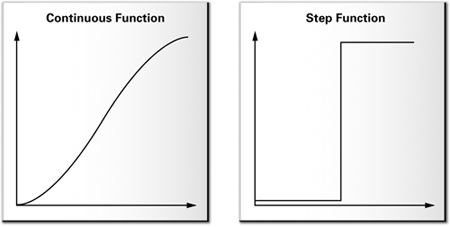
\includegraphics[width=1\linewidth]{fig9_4.jpg}
    \caption{Figure 9-4 A Continuous Function vs. a Step Function}
    \label{fig:9-4}
\end{figure}

Based on this principle, the diffuse part of a toon shader takes the $N$ dot $L$ part of the diffuse lighting calculation and classifies it as "bright" or "dark." You can choose the thresholds that you prefer, to get a "look" that you like.

To map $N$ dot $L$ values from a continuous range to a step function, use a texture lookup. Similar to the way you used a normalization cube map to encode a "normalize" function in Chapter 8, you can use a 1D texture to apply a step function. In this case, a 1D texture suffices because $N$ dot $L$ is a scalar. Figure \ref{fig:9-5} shows an example of a 1D texture that is two texels wide, along with the step function that it represents.

\begin{figure}
    \centering
    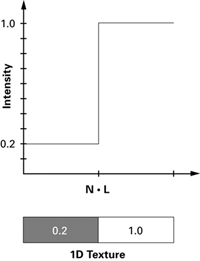
\includegraphics[width=0.5\linewidth]{fig9_5.jpg}
    \caption{Figure 9-5 Encoding a Step Function in a 1D Texture}
    \label{fig:9-5}
\end{figure}

Assuming that the application passes a texture called \textbf{diffuseRamp} to your toon shader, it's easy to apply a step function to the diffuse lighting:

\FloatBarrier
\begin{lstlisting}
diffuseLighting = tex1D(diffuseRamp, diffuseLighting);
\end{lstlisting}
\FloatBarrier

The old diffuse lighting value is replaced with the corresponding value from the step function. (Assume for now that no filtering is performed on the 1D texture. This ensures that the queried texture has only two distinct values, producing the sharp step function.)

\subsection*{Specular Highlights}

Handling the specular component is similar to handling the diffuse component. The idea is to apply a step function to the specular highlights, so that instead of having a gradual variation in strength, each highlight either exists or does not. This time, an application-specified texture called \textbf{specularRamp} provides the step function:

\FloatBarrier
\begin{lstlisting}
specularLighting = tex1D(specularRamp,
                         specularLighting);
\end{lstlisting}
\FloatBarrier

\subsection*{Silhouette Outlining}

Finally, you need to outline the objects. To do this, you need to find pixels that lie on the objects' silhouettes and color them with the outline color (normally black).

An easy way to find the silhouettes of objects is to use $N$ dot $V$ as a measuring stick. Just as $N$ dot $L$ measures how much light a surface receives, $N$ dot $V$ measures how much surface is visible from the current viewpoint. Recall that when you were calculating lighting for a point, the point was lit when $N$ dot $L$ was positive, and it was shadowed when $N$ dot $L$ was negative.

Similarly, a point is visible when $N$ dot $V$ is positive, and hidden when $N$ dot $V$ is negative. Points at which $N$ dot $V$ is close to zero represent transitions from visible to hidden—these are the points on or close to an object's silhouette. Once again, a 1D texture applies the step function:

\FloatBarrier
\begin{lstlisting}
   // Calculate edge color
   float edge = max(dot(N, V), 0);
   edge = tex1D(edgeRamp, edge);
\end{lstlisting}
\FloatBarrier
   
\subsection*{Addressing Aliasing}

The approach that we just described does create a toon-shaded effect, but it is prone to flickering artifacts (caused by aliasing) during animation. Why? Because the diffuse, specular, and edge tests are too strict: their results tend to fluctuate considerably as the object moves. This is a natural consequence of using a step function, whose value jumps abruptly when the function value changes.

To address this problem, you can create a larger 1D texture (for each test) that encodes a smoother transition. For example, you might use a texture that is 16 texels wide, and encode additional in-between steps in the middle 4 texels. Then, you can turn on bilinear texture filtering, which will smooth the transition automatically. The example in the accompanying software framework produces more visually pleasing results by using this approach.

\subsection{9.2.3 Putting It All Together}

Examples 9-3 and 9-4 show the complete programs and put the preceding discussion into a concrete form.

\FloatBarrier
\begin{lstlisting}[caption=Example 9-3. The \textbf{C9E3v_toonShading} Vertex Program]
void C9E3v_toonShading(float4 position : POSITION,
                       float3 normal   : NORMAL,

                   out float4 oPosition   : POSITION,
                   out float  diffuseLight  : TEXCOORD0,
                   out float  specularLight : TEXCOORD1,
                   out float  edge          : TEXCOORD2,

               uniform float3 lightPosition,
               uniform float3 eyePosition,
               uniform float  shininess,
               uniform float4x4 modelViewProj)
{
      oPosition = mul(modelViewProj, position);

  // Calculate diffuse lighting
  float3 N = normalize(normal);
  float3 L = normalize(lightPosition - position.xyz);
  diffuseLight = max(dot(N, L), 0);

  // Calculate specular lighting
  float3 V = normalize(eyePosition - position.xyz);
  float3 H = normalize(L + V);
  specularLight = pow(max(dot(N, H), 0), shininess);
  if (diffuseLight <= 0) specularLight = 0;

  // Perform edge detection
  edge = max(dot(N, V), 0);
}
\end{lstlisting}
\FloatBarrier

\FloatBarrier
\begin{lstlisting}[caption=Example 9-4. The \textbf{C9E4f_toonShading} Fragment Program]
void C9E4f_toonShading(float diffuseLight : TEXCOORD0,
                       float specularLight: TEXCOORD1,
                       float edge         : TEXCOORD2,

                   out float4 color : COLOR,

               uniform float4 Kd,
               uniform float4 Ks,
               uniform sampler1D diffuseRamp,
               uniform sampler1D specularRamp,
               uniform sampler1D edgeRamp)
{
  // Apply step functions
  diffuseLight = tex1D(diffuseRamp, diffuseLight).x;
  specularLight = tex1D(specularRamp, specularLight).x;
  edge = tex1D(edgeRamp, edge).x;

  // Compute the final color
  color = edge * (Kd * diffuseLight +
                  Ks * specularLight);
}
\end{lstlisting}
\FloatBarrier

\subsection{9.2.4 Problems with This Technique}

The method we've described for toon shading is simple to implement, but it has a significant drawback: it works well only for curved objects. This is because the program relies on a gradual fall-off of $N$ dot $V$ to find silhouette edges. When objects have sharp edges, $N$ dot $V$ suddenly changes at the boundary, immediately causing the outline to turn completely black.

A common way to get around this problem is to use a two-pass approach. First, draw a version of the model that is slightly expanded along its normals. Draw this geometry in black (or whatever color you want for the outline). Next, draw the remaining geometry as usual, using the toon shader but omitting the outline calculation. The result will be a rendering that has a toon-shaded appearance internally and a clear shell that defines each object's outline. Unfortunately, this approach only addresses silhouette edges, not internal edges.

Another solution is to perform edge detection in image space. This approach lets you find internal edges and ensure uniform edge widths. However, adding this analysis increases the cost of the shader.

\section{9.3 Projective Texturing}

When people refer to "texturing," they're usually talking about explicitly assigning texture coordinates to apply a texture onto a surface. However, this isn't the only way to use textures. In this section, you'll learn how textures can be projected onto surfaces, as if from a slide projector. Naturally, this technique is called \textit{projective texturing}.

Figure \ref{fig:9-6} shows an example of projective texturing. The scene consists of a plane, along with two objects—a box and a sphere—floating above it. The projector is almost directly above the objects, and is projecting the image of a demon down onto the scene. Notice that there is no notion of objects "blocking" light. For example, the demon's eye and nose appear on both the sphere and on the plane beneath it. Similarly, the demon's teeth appear on the box and on the plane. In its basic form, projective texturing does not account for the shadowing relationships between objects. The reasons for this will be clearer when you learn how projective texturing works. (The exercises at the end of this chapter explore one solution to this problem.)

\begin{figure}
    \centering
    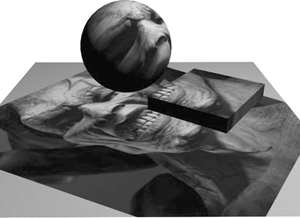
\includegraphics[width=0.75\linewidth]{fig9_6.jpg}
    \caption{Figure 9-6 Projective Texturing}
    \label{fig:9-6}
\end{figure}

\subsection{9.3.1 How Projective Texturing Works}

So how does projective texturing work? A projective texture is just like an ordinary texture—the only difference is in how the texture is applied to geometry. Like regular texturing, projective texturing requires every triangle in your scene to have the appropriate texture coordinates. If you get the texture coordinates right, you'll end up with the correct part of the light's texture on each triangle. The trick is assigning the correct coordinates to the various polygons.

Remember the discussion in Chapter 4, where we went through the various transformations in the graphics pipeline? Many of these concepts apply to projective texturing.

We started with object-space coordinates for each triangle and applied a series of transformations to map the vertices into a sequence of coordinate systems. The transformations projected the object-space vertices into window space, so that the triangles could be rasterized and displayed in the viewport. If you think of the viewport as a texture, it's evident that you ended up mapping each vertex to a texel on the texture.

Projective texturing works in much the same way. By applying a sequence of transformations, you map object-space coordinates into a 2D space (a texture), and you find out where each vertex maps to on the texture. Then you assign this position as the texture coordinate for the vertex, and apply the appropriate piece of the texture to each triangle as it is rendered.

\subsection*{Comparing Transformations}

Figure \ref{fig:9-7} illustrates the parallel between transformations in a conventional pipeline and those in projective texturing.

\begin{figure}
    \centering
    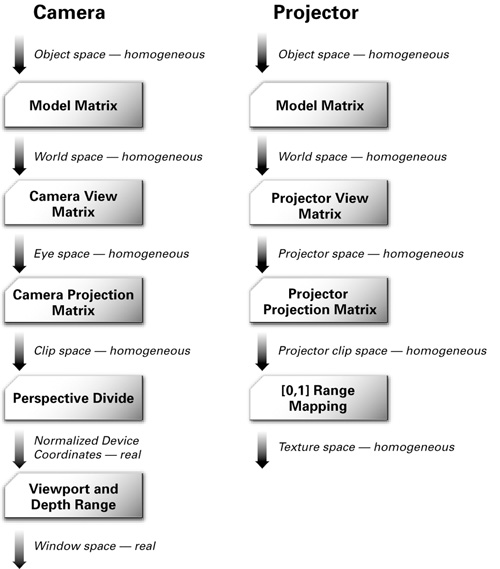
\includegraphics[width=0.75\linewidth]{fig9_7.jpg}
    \caption{Figure 9-7 Transformations for a Conventional Camera vs. Those for a Projector}
    \label{fig:9-7}
\end{figure}

On the left is the sequence of transformations in the conventional pipeline (for a typical "camera"), and on the right is the sequence of transformations for projective texturing. Notice that on the right side, the texture coordinates remain in homogeneous space. If you're wondering what "homogeneous space" means for texture coordinates, don't worry. That's what you're about to learn.

\subsection*{Homogeneous Texture Coordinates}

When texture coordinates are used, they're usually two-dimensional and nonprojective. Conventional 2D textures are accessed using a pair of texture coordinates: the $s$ and $t$ texture coordinates. Sometimes, when a 3D texture is applied, the $r$ texture coordinate is used to index the texture's third dimension. You can think of the $s$, $t$, and $r$ texture coordinates in the same way that you think of $x$, $y$, and $z$ when you're dealing with homogeneous positions.

Just as homogeneous positions have a fourth component called $w$, homogeneous texture coordinates also have a fourth component, called $q$. This component allows you to express projections, rotations, translations, and scales in texture space, all with convenient 4 $\times$ 4 matrix multiplications.

When it's time to perform a projective texture lookup, the hardware takes the original texture coordinate set ($s$, $t$, $r$, $q$) and divides each component by $q$, giving ($s/q$, $t/q$, $r/q$, 1). This is analogous to the perspective division that takes place after the vertex program runs. After this division, the coordinates index correctly into a 2D or 3D texture.

It should be clear by now that the theory for projective texturing is very similar to that of the basic graphics pipeline. For example, when you specify just $s$ and $t$ texture coordinates, $q$ is assumed to be 1. This is just like specifying a position directly in clip space (with $w$ equal to 1), as you did in Chapter 2. The only difference is that projections are almost always used when dealing with positions, but projective texturing is used sparingly when dealing with texture coordinates.

\subsection{9.3.2 Implementing Projective Texturing}

Now it's time to put the theory into practice. If you understand the concepts, you'll find that you don't have to do much at all in Cg to make projective texturing work.

There are two operations that you have to take care of: calculating projective texture coordinates in the vertex program, and performing the projective texture lookup in the fragment program.

\subsection*{Calculating Texture Coordinates in the Vertex Program}

In some of our previous vertex programs, you dealt with nonprojective texturing and simply passed the application's texture coordinates to the fragment program.

For projective texturing, you don't use explicitly specified per-vertex texture coordinates from the application. Rather, you use a vertex program to compute texture coordinates from the object-space per-vertex positions automatically. In fixed-function vertex processing, this computation occurs when automatic texture generation (commonly called "texgen") is enabled. The great thing about implementing texture generation in the vertex program is that you know exactly what's going on.

Equation 9-2 shows the sequence of transformations that you have to implement in the vertex program for projective texturing. Remember, it's the same sequence you would use if the eye were at the light's position, but with one extra matrix tacked on. This matrix scales and biases the results into the [0, 1] range that is used to access textures. For efficiency, you'll probably want to concatenate the matrices into a single matrix. We will call this concatenated matrix the texture matrix.

\FloatBarrier
\begin{equationcaption}
$
\begin{bmatrix} s \\ t \\ r \\ q \\ \end{bmatrix}
=
\begin{bmatrix} 1/2 & & & 1/2 \\ & 1/2 & & 1/2 \\ & & 1/2 & 1/2 \\ & & & 1 \\ \end{bmatrix}
\begin{bmatrix} Light \\ Frustum \\ (projection) \\ Matrix \\ \end{bmatrix}
\begin{bmatrix} Light \\ View \\ (look at) \\ Matrix \\ \end{bmatrix}
\begin{bmatrix}  \\ Modeling \\ Matrix \\  \\ \end{bmatrix}
\begin{bmatrix} x_0 \\ y_0 \\ z_0 \\ w_0 \\ \end{bmatrix}
$
\caption{Equation 9-2 The Sequence of Transformations for Projective Texturing}
\end{equationcaption}
\FloatBarrier

Let's go through the transformations, to clarify what's going on. The vertices start in object coordinates.

\begin{enumerate}
\item \textbf{Multiply by the modeling matrix.} This applies any necessary modeling transformations to the vertices. The modeling matrix needs to be applied regardless of whether or not you're using projective texturing.
\item \textbf{Multiply by the light's viewing matrix.} This rotates and translates the vertices so that they are in the light's frame of reference.
\item \textbf{Multiply by the light's projection matrix.} This defines the light's frustum, including its field of view and aspect ratio.
\item \textbf{Scale and bias the results.} Following steps 1 to 3, the transformed vertex values range from -1 to 1. However, textures are indexed from 0 to 1, so the results have to be mapped to this range. This is done by multiplying the $x$, $y$, and $z$ components of the results by $1/2$ and then adding $1/2$. A single matrix multiplication accomplishes this mapping.
\end{enumerate}

Now you need to come up with the matrices, which is easy. You already have the modeling matrix, because it was used to create the modelview matrix in Chapter 4. The light's viewing and projection matrices are what you would use if you were to render a scene from the light's point of view. And the scale-and-bias matrix is simply a collection of constants.

\subsection{9.3.3 The Code for Projective Texturing}

Once you've made sure that your application is passing the correct texture matrix to the vertex program, you need to add only one line to the vertex and fragment programs.

In the vertex program, you have to calculate the projective texture coordinates from the object-space positions:

\FloatBarrier
\begin{lstlisting}
   float4 texCoordProj = mul(textureMatrix, position);
\end{lstlisting}
\FloatBarrier

The fragment program receives the interpolated four-component texture coordinate set. Prior to using the texture coordinate set to access a 2D texture, the \textbf{tex2Dproj} Standard Library routine first divides the $s$ and $t$ texture coordinates (the first and second components) by the $q$ texture coordinate (the fourth component):

\FloatBarrier
\begin{lstlisting}   
   float4 textureColor = tex2Dproj(projTexture,
                                   texCoordProj);
\end{lstlisting}
\FloatBarrier

Notice that the complete four-component texture coordinates are passed to \textbf{tex2Dproj}, with the $q$ component as the fourth component.

\subsection*{The Vertex Program}

Example 9-5 shows the complete vertex program for projective texturing.

\begin{lstlisting}[caption=Example 9-5. The \textbf{C9E5v_projTex} Vertex Program]
void C9E5v_projTex(float4 position : POSITION,
                   float3 normal   : NORMAL,

               out float4 oPosition       : POSITION,
               out float4 texCoordProj    : TEXCOORD0,
               out float4 diffuseLighting : COLOR,

           uniform float Kd,
           uniform float4x4 modelViewProj,
           uniform float3 lightPosition,
           uniform float4x4 textureMatrix)
{
  oPosition = mul(modelViewProj, position);

  // Compute texture coordinates for
  // querying the projective texture
  texCoordProj = mul(textureMatrix, position);

  // Compute diffuse lighting
  float3 N = normalize(normal);
  float3 L = normalize(lightPosition - position.xyz);
  diffuseLighting = Kd * max(dot(N, L), 0);
}
\end{lstlisting}

\subsubsection*{The Fragment Program}

Example 9-6 shows the corresponding fragment program.

\begin{lstlisting}[caption=Example 9-6. The \textbf{C9E6f_projTex} Fragment Program]
void C9E6f_projTex(float4 texCoordProj    : TEXCOORD0,
                   float4 diffuseLighting : COLOR,

               out float4 color : COLOR,

           uniform sampler2D projectiveMap)
{
  // Fetch color from the projective texture
  float4 textureColor = tex2Dproj(projectiveMap,
                                  texCoordProj);

  color = textureColor * diffuseLighting;
}
\end{lstlisting}

\subsection*{Notable Issues}

Projective texturing has two issues that you should be aware of. First, there are no occlusion checks. This means that the intuitive notion of triangles shadowing one another as with a real slide projector does not exist—the projective texture is applied to every triangle that is within the light's frustum. This behavior shouldn't come as a surprise, considering that the hardware simply transforms vertices according to the matrices that it's given, and uses the transformed locations to query a texture. As the hardware transforms each triangle, it has no knowledge of the triangle's relationship to any others.

The second issue is that back-projection artifacts can appear when the q coordinate is negative. \textit{Back-projection} refers to the texture being projected on surfaces that are behind the light source (or projector). On many older GPUs, the texture interpolators produce undefined results in this case.

There are several ways to avoid artifacts when $q$ is negative:
\begin{itemize}
\item Use culling to draw only geometry that is in front of the light source.
\item Use clip planes to remove geometry that is behind the light source.
\item Fold the back-projection factor into a 3D attenuation texture.
\item Use a fragment program to check when q is negative.
\end{itemize}

The first two solutions are tedious to implement; the fragment program solution is simple and efficient but requires an advanced fragment profile. Just check the value of the $q$ coordinate. If $q$ is negative, you can ignore the projective texture computation and output black. In this case, you can rewrite the texture lookup in \textbf{C9E6f_projTex} to read:

\FloatBarrier
\begin{lstlisting}
float4 textureColor = texCoordProj.w < 0 ?  // is q less than 0?
                      0 :                   // then zero
                      tex2Dproj(projTexture, texCoordProj);
                      // otherwise sample the texture
\end{lstlisting}
\FloatBarrier

\section{9.4 Shadow Mapping}

If you've used OpenGL or Direct3D, you know that lights in these APIs do not automatically cast shadows. There are lots of ways to compute shadows, but we're going to look at only one of the popular methods, called \textit{shadow mapping}. Figure \ref{fig:9-8} shows the effect of adding shadows to a simple scene. The shadows help to establish the relative locations of the sphere and the cube.

\begin{figure}
    \centering
    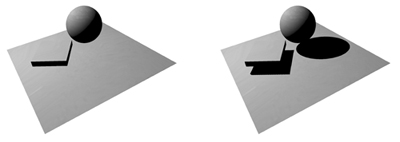
\includegraphics[width=1\linewidth]{fig9_8.jpg}
    \caption{Figure 9-8 Using Shadow Mapping to Add Shadows to a Scene}
    \label{fig:9-8}
\end{figure}

We cover shadow mapping for two reasons. First, it's based on the projective texturing concept that we just introduced. And second, the fragment programming capabilities of recent graphics hardware let you control shadow mapping more precisely than ever before.

Shadow mapping is a two-pass technique:

\begin{enumerate}
\item First, the scene is rendered from the light's point of view. The depth at each pixel of the resulting image is recorded in a "depth texture." (This texture is often called the \textit{shadow map}.)
\item Next, the scene is rendered from the eye position, but with the shadow map projected down from the light onto the scene using standard projective texturing. At each pixel, the depth sample (from the projected shadow map texture) is compared with the fragment's distance from the light. If the latter is greater, the pixel is not the closest surface to the light source. This means that the fragment is shadowed, and that it should not receive light during shading.
\end{enumerate}

Figure \ref{fig:9-9} illustrates the shadow mapping comparison. On the left panel of the figure, the point $P$ that is being shaded is in shadow, because the point's depth ($z_B$) is greater than the depth that is recorded in the shadow map ($z_A$). In contrast, the right panel of the figure shows a case where the point $P$ has the same depth as the recorded value in the shadow map. This means that there isn't any object between $P$ and the light source, so $P$ is not in shadow.

\begin{figure}
    \centering
    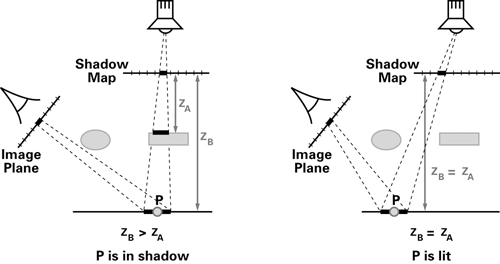
\includegraphics[width=1\linewidth]{fig9_9.jpg}
    \caption{Figure 9-9 The Shadow Mapping Depth Comparison}
    \label{fig:9-9}
\end{figure}

Shadow mapping uses the same setup that projective texturing uses, so the shadow map is indexed using ($s/q$, $t/q$). Because the light source is the center of projection for the shadow map, $r/q$ holds the distance from the light. Therefore, by comparing the shadow map texel depth at ($s/q$, $t/q$) with $r/q$, you can determine if the current pixel is lit or in shadow.

When you do a projective texture lookup on a shadow map, the hardware automatically takes care of the comparison for you: the \textbf{tex2Dproj} function returns a value that represents how "lit" the current pixel would be. That is, the \textbf{tex2Dproj} function returns a four-component vector of the form ($c$, $c$, $c$, 1), where $c$ is 0 if the pixel is in shadow, and 1 if the pixel is lit. You can then treat this vector as a color. If bilinear texture filtering is enabled, $c$ will range from 0 to 1 instead of being restricted to just the two values. Filtering is useful along the shadow boundaries, where the transition between being fully occluded to fully lit takes place. In these situations, the filtering helps make the shadow look softer, and reduces edge aliasing (jaggedness).

The following code sample shows how you would use a shadow map in a fragment program. In the example, the diffuse lighting is modulated by the result of the shadow map query:

\FloatBarrier
\begin{lstlisting}
   // Calculate diffuseLighting as usual

   // Fetch depth value from the shadow map
   float4 shadowCoeff;   // 0 means "in shadow",
                         // 1 means "not in shadow"
   shadowCoeff = tex2Dproj(shadowMap,
                           texCoordProj);

   float4 shadowedColor = shadowCoeff *
                          diffuseLighting;
\end{lstlisting}
\FloatBarrier

Notice that the code for the shadow map query is virtually identical to the code for the projective texture lookup in Example 9-6. To a Cg programmer, shadow maps are like other projective textures, except that instead of returning a texture color, \textbf{tex2Dproj} returns a value representing shadow coverage. The underlying hardware implementation automatically recognizes when a texture is a depth texture (instead of a color texture) and performs the shadow map comparison instead of an ordinary texture fetch.

\subsection*{Extensions}

Conventional shadow mapping with the fixed-function pipeline automatically handles the shadow map comparison for you. But with fragment programs, you can take full control of this operation and apply it to create new effects.

Shadow generation is a very difficult topic, and it has been the subject of many research papers and projects. The "Further Reading" section at the end of this chapter lists several sources that you can use to learn more about shadow mapping and other ways of generating shadows. As you experiment, you're likely to find new techniques that you can incorporate into your own projects to give them a unique look.

\section{9.5 Compositing}

The same fragment-processing power available for high-level shading of 3D surfaces can be usefully employed in 2D imaging as well. Applications such as painting programs and digital photo readers already make use of complex 2D processes. And most motion-picture uses of computer graphics now rely heavily on the ability to composite multiple images, sometimes from widely different sources, into a single final frame. Even games can benefit from fast, high-quality imaging effects, applied as a postprocess to their original 3D outputs.

Simple compositing has been around for many years, using the technique of alpha blending; this capability is present in both Direct3D and OpenGL. The technique is mostly used when rendering individual 3D polygons to a partially filled frame buffer, but it can also be used for 2D image processing. But the precision of alpha blending is limited to fixed-point math, and this limitation can sometimes lead to serious errors in the compositing process.

Recent GPUs have introduced floating-point offscreen buffers, permitting extremely complex compositing effects while essentially removing concerns about loss of precision. Floating-point buffers do not use hardware alpha blending, but instead depend on the fragment-shading pipeline. Floating-point buffers are brought back into the fragment pipeline as floating-point textures. Thus, we can combine images using fragment program operations, and then write out the final processed result to the frame buffer. Fragment programs permit us to perform not only all of the many combinations previously available in alpha blending, but also any fragment-oriented processes we can imagine.

\begin{framed}
CineFX

The CineFX architecture provides four-component floating-point math operations and frame buffer formats. Each component is processed and stored as an industry-standard (IEEE) 32-bit floating-point value.
\end{framed}

\subsection{9.5.1 Mapping Input to Output Pixels}

When using fragment programs to perform 2D image processing, we are actually still doing 3D imaging! We render polygons directly aligned with the screen, and covering the screen. We apply our 2D fragment programs directly to this surface.

The typical way to cover the screen is with a simple screen-aligned rectangle (two triangles). If we define a 3D unit-sized square, ranging from -0.5 to 0.5 in $x$ and $y$ and with $z = 0$ for all points, then the Cg vertex program in Example 9-7 will align it with the screen.

Note that depending on the graphics API that you use, you may have to add offsets to align images correctly. For instance, in Example 9-7, \textbf{0.5/imgWidth} and \textbf{0.5/imgHeight} are tiny offsets that align images for Direct3D. This is necessary because in Direct3D, texture coordinates address the center of each texel, not one corner. The slight shift is seldom visible to the naked eye, but it can create numerous problems if you attempt to combine the results of multiple imaging passes. Each pass, if misaligned, will be offset a half-texel, which can create some cool effects of its own, but is generally undesirable if unintended!

\subsection{9.5.2 Basic Compositing Operations}

Once we have aligned a screen-shaped surface and placed texture coordinates onto it, we can combine any input images we like.

To copy an image directly to the screen (potentially rescaling it as you go), use a very simple fragment program shown in Example 9-8 (which includes a tint color, just for fun).

\begin{lstlisting}[caption=Example 9-7. The \textbf{C9E7v_screenAlign} Vertex Program]
void C9E7v_screenAlign(float3 position : POSITION,
                       float4 texCoord : TEXCOORD0,

                   out float4 oPosition : POSITION,
                   out float4 oTexCoord : TEXCOORD0,

               uniform float imgWidth,
               uniform float imgHeight)
{
  float4 screen = float4(position.x, position.y,
                         2.0, 2.0);
  oPosition = screen;
  oTexCoord = float4(0.5 * (1.0 + screen.x/screen.w) +
                     (0.5/imgWidth),
                     0.5 * (1.0 + screen.y/screen.w) +
                     (0.5/imgHeight),
                     0.0,
                     1.0);
}
\end{lstlisting}

\begin{lstlisting}[caption=Example 9-8. The \textbf{C9E8f_tint} Fragment Program]
void C9E8f_tint(float3 position : POSITION,
                float2 texCoord : TEXCOORD0,

            out float4 result   : COLOR,

        uniform sampler2D colorMap,
        uniform float4 tintColor)
{
  result = tintColor * tex2D(colorMap, texCoord);
}
\end{lstlisting}

Example 9-9 adds a second image to open up the realm of compositing.

\begin{framed}
CineFX

Note that Example 9-9 and the other compositing examples that follow work only on advanced profiles, though you can easily rewrite them for basic profiles by replicating the texture coordinate set. Then, you would access each sampler with its own texture coordinate set (even though the two sets of texture coordinates would in fact be identical), which is allowed in basic profiles.
\end{framed}

\begin{lstlisting}[caption=Example 9-9. The \textbf{C9E9f_a_over_b} Fragment Program]
void C9E9f_a_over_b(float3 position : POSITION,
                    float2 texCoord : TEXCOORD0,

                out float4 result   : COLOR,

            uniform sampler2D imageA,
            uniform sampler2D imageB)
{
  float4 aPixel = tex2D(imageA, texCoord);
  float4 bPixel = tex2D(imageB, texCoord);
  result = (aPixel.w * aPixel) +
           ((1.0 - aPixel.w) * bPixel);
}
\end{lstlisting}

This fragment program implements a typical compositing "over" operator, based on input values that are not premultiplied (sometimes called "nonpremultiplied"). In other words, the RGB portion of \textbf{imageA}'s pixels isn't already integrated with the alpha. Sometimes, particularly when dealing with images that have been antialiased, the alpha and RGB components have already been scaled, or premultiplied. If \textbf{imageA} had been premultiplied by alpha, we would change the equation slightly:

\FloatBarrier
\begin{lstlisting}
   float4 result = aPixel + ((1.0 - aPixel.w) * bPixel);
\end{lstlisting}
\FloatBarrier

Note that since we've ignored the alpha for \textbf{imageB} in this case, it doesn't matter if \textbf{imageB} is premultiplied or postmultiplied—unless you plan to use the result of the operation in further compositing passes. Beware of mixing premultiplied and nonpremultiplied images!

Using only slight variations, you can create other standard compositing operations, such as the following:

\begin{itemize}
\item \textbf{In:} Show \textbf{imageA} only when it overlaps with \textbf{imageB}, as shown in Example 9-10.
\item \textbf{Out:} Show \textbf{imageA} only when it's \textit{not} overlapping \textbf{imageB}, as shown in Example 9-11.
\item \textbf{Dissolve:} Blend the two images (also called "additive blend" or just "mix" in compositing circles), as shown in Example 9-12.
\end{itemize}

Combining these simple pixel-to-pixel operations can create a near-infinite variety of effects. For example, you may want to overlay \textbf{imageB} with \textbf{imageA} but apply a dissolve-like \textbf{lerp} to \textbf{imageA}'s alpha channel. You can use channel swizzles to create new "chroma-key" values for alpha on the fly. You can also perform useful alterations to the color and look of your input images before and after direct compositing. Color alterations of the input and final images can give you access to a wide range of image effects, applied in 2D, without having to change your underlying 3D models and rendering pipeline.

\begin{lstlisting}[caption=Example 9-10. The \textbf{C9E10f_a_in_b} Fragment Program]
void C9E10f_a_in_b(float3 position : POSITION,
                   float2 texCoord : TEXCOORD0,

               out float4 result   : COLOR,

           uniform sampler2D imageA,
           uniform sampler2D imageB)
{
  float4 aPixel = tex2D(imageA, texCoord);
  float4 bPixel = tex2D(imageB, texCoord);
  result = bPixel.w * aPixel;
}
\end{lstlisting}

\begin{lstlisting}[caption=Example 9-11. The \textbf{C9E11f_a_out_b} Fragment Program]
void C9E11f_a_out_b(float3 position : POSITION,
                    float2 texCoord : TEXCOORD0,

                out float4 result   : COLOR,

            uniform sampler2D imageA,
            uniform sampler2D imageB)
{
  float4 aPixel = tex2D(imageA, texCoord);
  float4 bPixel = tex2D(imageB, texCoord);
  result = (1.0 - bPixel.w) * aPixel;
}
\end{lstlisting}

\begin{lstlisting}[caption=Example 9-12. The \textbf{C9E12f_a_dissolve_b} Fragment Program]
void C9E12f_a_dissolve_b(float3 position : POSITION,
                         float2 texCoord : TEXCOORD0,

                     out float4 result   : COLOR,

                 uniform sampler2D imageA,
                 uniform sampler2D imageB,
                 uniform float dissolve)
{
  float4 aPixel = tex2D(imageA, texCoord);
  float4 bPixel = tex2D(imageB, texCoord);
  result = lerp(aPixel, bPixel, dissolve);
}
\end{lstlisting}

\section{9.6 Exercises}
\begin{itemize}
\item \textbf{Try this yourself:} Depth cueing is a nonphotorealistic technique that is similar to fog. Both techniques attenuate apparent color with distance from the viewer. Unlike uniform fog, which uses an exponential function, depth cueing uses a simpler linear attenuation. Depth cueing helps a CAD designer viewing complex wireframe models to tell which lines are closer and which are farther away. Change the C9E1f_fog\textbf{ }and \textbf{C9E2v_fog} examples to implement depth cueing. \textit{Hint:} For example, OpenGL supports depth cueing through its \textbf{GL_LINEAR} fog mode. In this mode, the $f$ in Equation 9-1 is computed this way, with no exponential:

\FloatBarrier
$
f=max\left( 0,min\left( 1,\frac{e-Z}{e-s}\right) \right)
$
\FloatBarrier

where $s$ is the location where the fog starts in eye space (\textbf{GL_FOG_START} in OpenGL) and $e$ is where the fog ends (\textbf{GL_FOG_END} in OpenGL).

\item \textbf{Answer this:} Describe a uniform fog situation where computing the distance per-vertex with the Euclidean distance function \textbf{length} would create artifacts. \textit{Hint:} Think about a situation where two vertices could have the same distance from the eye but be far apart from each other.

\item \textbf{Try this yourself:} Modify the \textbf{C9E4f_toonShading} example so that, rather than using two 1D textures—one for diffuse and one for specular—the program uses a single 2D texture index with the diffuse contribution for s and the specular contribution for $t$. You will have to create an appropriate 2D texture.

\item \textbf{Try this yourself:} Use projective texturing to create a spotlight pattern in the shape of a blurred five-point star. Combine the spotlight attenuation term from projective texturing with a diffuse and specular lighting model from Chapter 5.

\item \textbf{Try this yourself:} Try combining shadow mapping with the results from Exercise 4.

\item \textbf{Try this yourself:} You saw in Section 9.5.1 that remapping an image to match exactly the output screen can be performed by a very small vertex program to define $s-t$ texture coordinates. Extend such a vertex program to include standard 2D affine transformations to the 2D image, such as scaling, translation, and rotation.
\end{itemize}

\section{9.7 Further Reading}

To learn more about fog, read the "Atmospheric Models" chapter by Ken Musgrave, Larry Gritz, and Steven Worley in \textit{Texturing and Modeling: A Procedural Approach, Second Edition} (Academic Press, 1998), edited by David S. Ebert. The classic computer graphics topic on atmospheric effects is Victor Klassen's "Modeling the Effect of the Atmosphere on Light," which appeared in a 1987 issue of \textit{ACM Transactions on Graphics}.

Fog is more interesting when you relax the restriction of having uniform fog color and density. Justin Legakis presented a technical sketch at SIGGRAPH 1998, called "Fast Multi-Layer Fog" (ACM Press), in which he assumed that fog density varies with elevation.

Tomoyuki Nishita and his collaborators published a host of papers on natural phenomena, particularly atmospheric effects such as shafts of light. Much of their work could be easily adapted for use in Cg programs. His Web site is \textbf{http://nis-lab.is.s.u-tokyo.ac.jp/~nis}.

In 2001, Amy and Bruce Gooch wrote \textit{Non-Photorealistic Rendering} (A. K. Peters), which describes cartoon rendering in more detail, along with many other nonphotorealistic rendering techniques. Thomas Strothotte and Stefan Schlechtweg wrote \textit{Non-Photorealistic Computer Graphics: Modeling, Rendering and Animation} (Morgan Kaufmann, 2002).

Mark Segal, Carl Korobkin, Rolf van Widenfelt, Jim Foran, and Paul Haeberli introduced projective texturing for graphics hardware in their SIGGRAPH 1992 paper "Fast Shadows and Lighting Effects Using Texture Mapping" (ACM Press). This paper also describes hardware texture mapping as an extension of projective texturing.

Lance Williams first described shadow mapping in his classic SIGGRAPH 1978 paper "Casting Curved Shadows on Curved Surfaces" (ACM Press). William Reeves, David Salesin, and Robert Cook described their work on shadow maps at Pixar in their SIGGRAPH 1987 paper "Rendering Antialiased Shadows with Depth Maps" (ACM Press).

OpenGL 1.4 standardized shadow mapping for graphics hardware in 2002. Cass Everitt, Ashu Rege, and Cem Cebenoyan published "Hardware Shadow Mapping" for OpenGL and Direct3D in 2002. The white paper is available on NVIDIA's Developer Web site (\textbf{developer.nvidia.com}).

"A Survey of Shadow Algorithms," by Andrew Woo, Pierre Poulin, and Alain Fournier, is an excellent paper to learn more about shadows and shadow algorithms. The paper appeared in \textit{IEEE Computer Graphics and Applications} in 1990.

Thomas Porter and Tom Duff published "Compositing Digital Images" (ACM Press) at SIGGRAPH 1984 and introduced compositing to the graphics community. More recently, Ron Brinkmann published \textit{The Art and Science of Digital Compositing} (Morgan Kaufmann, 1999).

\end{document}